\documentclass[12pt,a4paper]{report}
\usepackage[utf8]{inputenc}
\usepackage[english]{babel}
\usepackage{amsmath}
\usepackage{amsfonts}
\usepackage{amssymb}
\usepackage{graphicx}
\usepackage{cite}
\usepackage[left=2cm,right=2cm,top=2cm,bottom=2cm]{geometry}
\author{Eva María Urbano González}
\title{Encryption}
\begin{document}
\maketitle
\chapter{Encryption}
\section{Is encryption necessary in satellites?}
\textit{In the light of latest intrusions into satellite data the demand to protect the sensitive and valuable data transmitted from satellites to ground has increase and hence the need to use encryption on-board}\cite{Sayeda2007}. 
Currently, only few satellites are equipped with on-board encryption to protect the data transmitted to ground satation, but more and more organizations are planning to have on-board encryption as a security mesure.
\section{Satellite On-Board Encryption}
Due to limited computational resources on-board, the encryption technology used in spacecrafts is very different that the one used in terrestrial systems. In the following table we can see a brief description of each of the existing planned satellites with encryption on-board.\\
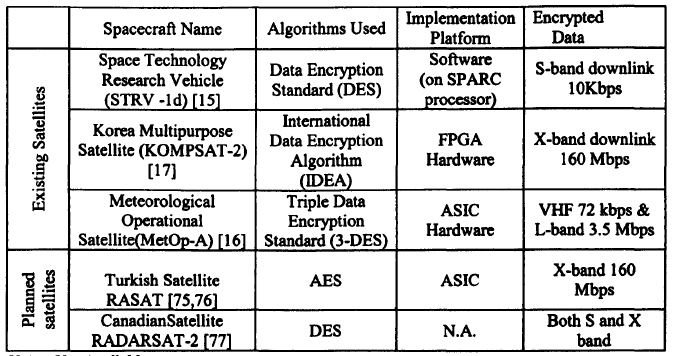
\includegraphics[scale=1]{tableonboardecryption.png} \\
\section{Security services for Uplink Commands}
The uplink or telecommand should \textbf{always} be checked for integrity and authentication in order to protect the satellite from being taken over by unauthorized people. There must exist and authentication and integrity block which provides protection to the satellite by ensuring that the on-board data handling system receive unmodified telecommands from authorized ground station. Data authentication is usually achieved by appending an extra unit of information to the original message (the digital signature).  The digital signature identifies the origin of the data. Many digital signature generation mechanisms require the use of an asymmetric cryptographic algorithm where senter and receiver do not hold the same cryptographic keys. An integrity service is used to ensure that unauthorized users have not manipulated the data in any way. Integrity of data is achieved by appending an Integrity Check Value (ICV) to the data structure in a manner similar to the way  a digital signature is appended, but in this case thee ICV is always a function of the data itself. All these telecommands may also be encrypted by ground station depending on the level of security required. 
Here we can see an example of a block diagram of the the on-board security architecture. In this case the satellite is an small EO satellite. \\
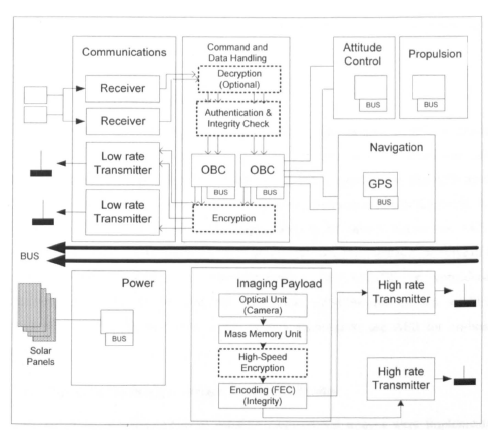
\includegraphics[scale=1]{exampleauthenti.png}  
\section{Security services for downlink data}
This information is related with satellite health, control information (AOCS), temperature, etc.
\section{Encryption of Payload information}
The usual algorithms to use is AES. The most popular modes of AES are: ECB, CBC, OFB, CFB, CTR. They are carried out using a purpose-build software simulator developed in JAVA. 
\bibliographystyle{plain}
\bibliography{library}
\end{document}
